%  LaTeX support: latex@mdpi.com 
%  For support, please attach all files needed for compiling as well as the log file, and specify your operating system, LaTeX version, and LaTeX editor.

%=================================================================
\documentclass[remotesensing,article,submit,pdftex,moreauthors]{Definitions/mdpi} 

%--------------------
% Class Options:
%--------------------
%----------
% journal
%----------
% Choose between the following MDPI journals:
% acoustics, actuators, addictions, admsci, adolescents, aerobiology, aerospace, agriculture, agriengineering, agrochemicals, agronomy, ai, air, algorithms, allergies, alloys, analytica, analytics, anatomia, animals, antibiotics, antibodies, antioxidants, applbiosci, appliedchem, appliedmath, applmech, applmicrobiol, applnano, applsci, aquacj, architecture, arm, arthropoda, arts, asc, asi, astronomy, atmosphere, atoms, audiolres, automation, axioms, bacteria, batteries, bdcc, behavsci, beverages, biochem, bioengineering, biologics, biology, biomass, biomechanics, biomed, biomedicines, biomedinformatics, biomimetics, biomolecules, biophysica, biosensors, biotech, birds, bloods, blsf, brainsci, breath, buildings, businesses, cancers, carbon, cardiogenetics, catalysts, cells, ceramics, challenges, chemengineering, chemistry, chemosensors, chemproc, children, chips, cimb, civileng, cleantechnol, climate, clinpract, clockssleep, cmd, coasts, coatings, colloids, colorants, commodities, compounds, computation, computers, condensedmatter, conservation, constrmater, cosmetics, covid, crops, cryptography, crystals, csmf, ctn, curroncol, cyber, dairy, data, ddc, dentistry, dermato, dermatopathology, designs, devices, diabetology, diagnostics, dietetics, digital, disabilities, diseases, diversity, dna, drones, dynamics, earth, ebj, ecologies, econometrics, economies, education, ejihpe, electricity, electrochem, electronicmat, electronics, encyclopedia, endocrines, energies, eng, engproc, entomology, entropy, environments, environsciproc, epidemiologia, epigenomes, est, fermentation, fibers, fintech, fire, fishes, fluids, foods, forecasting, forensicsci, forests, foundations, fractalfract, fuels, future, futureinternet, futurepharmacol, futurephys, futuretransp, galaxies, games, gases, gastroent, gastrointestdisord, gels, genealogy, genes, geographies, geohazards, geomatics, geosciences, geotechnics, geriatrics, grasses, gucdd, hazardousmatters, healthcare, hearts, hemato, hematolrep, heritage, higheredu, highthroughput, histories, horticulturae, hospitals, humanities, humans, hydrobiology, hydrogen, hydrology, hygiene, idr, ijerph, ijfs, ijgi, ijms, ijns, ijpb, ijtm, ijtpp, ime, immuno, informatics, information, infrastructures, inorganics, insects, instruments, inventions, iot, j, jal, jcdd, jcm, jcp, jcs, jcto, jdb, jeta, jfb, jfmk, jimaging, jintelligence, jlpea, jmmp, jmp, jmse, jne, jnt, jof, joitmc, jor, journalmedia, jox, jpm, jrfm, jsan, jtaer, jvd, jzbg, kidneydial, kinasesphosphatases, knowledge, land, languages, laws, life, liquids, literature, livers, logics, logistics, lubricants, lymphatics, machines, macromol, magnetism, magnetochemistry, make, marinedrugs, materials, materproc, mathematics, mca, measurements, medicina, medicines, medsci, membranes, merits, metabolites, metals, meteorology, methane, metrology, micro, microarrays, microbiolres, micromachines, microorganisms, microplastics, minerals, mining, modelling, molbank, molecules, mps, msf, mti, muscles, nanoenergyadv, nanomanufacturing,\gdef\@continuouspages{yes}} nanomaterials, ncrna, ndt, network, neuroglia, neurolint, neurosci, nitrogen, notspecified, %%nri, nursrep, nutraceuticals, nutrients, obesities, oceans, ohbm, onco, %oncopathology, optics, oral, organics, organoids, osteology, oxygen, parasites, parasitologia, particles, pathogens, pathophysiology, pediatrrep, pharmaceuticals, pharmaceutics, pharmacoepidemiology,\gdef\@ISSN{2813-0618}\gdef\@continuous pharmacy, philosophies, photochem, photonics, phycology, physchem, physics, physiologia, plants, plasma, platforms, pollutants, polymers, polysaccharides, poultry, powders, preprints, proceedings, processes, prosthesis, proteomes, psf, psych, psychiatryint, psychoactives, publications, quantumrep, quaternary, qubs, radiation, reactions, receptors, recycling, regeneration, religions, remotesensing, reports, reprodmed, resources, rheumato, risks, robotics, ruminants, safety, sci, scipharm, sclerosis, seeds, sensors, separations, sexes, signals, sinusitis, skins, smartcities, sna, societies, socsci, software, soilsystems, solar, solids, spectroscj, sports, standards, stats, std, stresses, surfaces, surgeries, suschem, sustainability, symmetry, synbio, systems, targets, taxonomy, technologies, telecom, test, textiles, thalassrep, thermo, tomography, tourismhosp, toxics, toxins, transplantology, transportation, traumacare, traumas, tropicalmed, universe, urbansci, uro, vaccines, vehicles, venereology, vetsci, vibration, virtualworlds, viruses, vision, waste, water, wem, wevj, wind, women, world, youth, zoonoticdis 
% For posting an early version of this manuscript as a preprint, you may use "preprints" as the journal. Changing "submit" to "accept" before posting will remove line numbers.

%---------
% article
%---------
% The default type of manuscript is "article", but can be replaced by: 
% abstract, addendum, article, book, bookreview, briefreport, casereport, comment, commentary, communication, conferenceproceedings, correction, conferencereport, entry, expressionofconcern, extendedabstract, datadescriptor, editorial, essay, erratum, hypothesis, interestingimage, obituary, opinion, projectreport, reply, retraction, review, perspective, protocol, shortnote, studyprotocol, systematicreview, supfile, technicalnote, viewpoint, guidelines, registeredreport, tutorial
% supfile = supplementary materials

%----------
% submit
%----------
% The class option "submit" will be changed to "accept" by the Editorial Office when the paper is accepted. This will only make changes to the frontpage (e.g., the logo of the journal will get visible), the headings, and the copyright information. Also, line numbering will be removed. Journal info and pagination for accepted papers will also be assigned by the Editorial Office.

%------------------
% moreauthors
%------------------
% If there is only one author the class option oneauthor should be used. Otherwise use the class option moreauthors.

%---------
% pdftex
%---------
% The option pdftex is for use with pdfLaTeX. Remove "pdftex" for (1) compiling with LaTeX & dvi2pdf (if eps figures are used) or for (2) compiling with XeLaTeX.

%=================================================================
% MDPI internal commands - do not modify
\firstpage{1} 
\makeatletter 
\setcounter{page}{\@firstpage} 
\makeatother
\pubvolume{1}
\issuenum{1}
\articlenumber{0}
\pubyear{2024}
\copyrightyear{2024}
%\externaleditor{Academic Editor: Firstname Lastname}
\datereceived{ } 
\daterevised{ } % Comment out if no revised date
\dateaccepted{ } 
\datepublished{ } 
%\datecorrected{} % For corrected papers: "Corrected: XXX" date in the original paper.
%\dateretracted{} % For corrected papers: "Retracted: XXX" date in the original paper.
\hreflink{https://doi.org/} % If needed use \linebreak
%\doinum{}
%\pdfoutput=1 % Uncommented for upload to arXiv.org
%\CorrStatement{yes}  % For updates


%=================================================================
% Add packages and commands here. The following packages are loaded in our class file: fontenc, inputenc, calc, indentfirst, fancyhdr, graphicx, epstopdf, lastpage, ifthen, float, amsmath, amssymb, lineno, setspace, enumitem, mathpazo, booktabs, titlesec, etoolbox, tabto, xcolor, colortbl, soul, multirow, microtype, tikz, totcount, changepage, attrib, upgreek, array, tabularx, pbox, ragged2e, tocloft, marginnote, marginfix, enotez, amsthm, natbib, hyperref, cleveref, scrextend, url, geometry, newfloat, caption, draftwatermark, seqsplit
% cleveref: load \crefname definitions after \begin{document}

%=================================================================
% Please use the following mathematics environments: Theorem, Lemma, Corollary, Proposition, Characterization, Property, Problem, Example, ExamplesandDefinitions, Hypothesis, Remark, Definition, Notation, Assumption
%% For proofs, please use the proof environment (the amsthm package is loaded by the MDPI class).

%=================================================================
% Full title of the paper (Capitalized)
\Title{Generative Simplex Mapping: Nonlinear Endmember Extraction and Unmixing for Hyperspectral Imagery}

% MDPI internal command: Title for citation in the left column
\TitleCitation{Generative Simplex Mapping: Nonlinear Endmember Extraction and Unmixing for Hyperspectral Imagery}

% Author Orchid ID: enter ID or remove command
\newcommand{\orcidauthorA}{0000-0002-5910-0183} % John
\newcommand{\orcidauthorB}{0000-0003-4265-9543} % David

% Authors, for the paper (add full first names)
\Author{John Waczak \orcidA{} and David J. Lary *\orcidB{}}

%\longauthorlist{yes}

% MDPI internal command: Authors, for metadata in PDF
\AuthorNames{John Waczak and David J. Lary}

% MDPI internal command: Authors, for citation in the left column
\AuthorCitation{Waczak, J.; Lary, D.J.}
% If this is a Chicago style journal: Lastname, Firstname, Firstname Lastname, and Firstname Lastname.

% Affiliations / Addresses (Add [1] after \address if there is only one affiliation.)
% Affiliations / Addresses (Add [1] after \address if there is only one affiliation.)
\address[1]{%
Hanson Center for Space Sciences, University of Texas at Dallas, Richardson, TX 75080, USA;  john.waczak@utdallas.edu (J.W.)}

% Contact information of the corresponding author
\corres{\hangafter=1 \hangindent=1.05em \hspace{-0.82em}Correspondence: david.lary@utdallas.edu} %; Tel.: (optional; include country code; if there are multiple corresponding authors, add author initials) +xx-xxxx-xxx-xxxx (F.L.)}

%\simplesumm{} % Simple summary

%\conference{} % An extended version of a conference paper

% Abstract (Do not insert blank lines, i.e. \\) 
\abstract{\textcolor{red}{UPDATE ME!}}

% Keywords
\keyword{Endmember Extraction; Spectral Unmixing; Hyperspectral Imaging; Unsupervised Machine Learning} 


%%%%%%%%%%%%%%%%%%%%%%%%%%%%%%%%%%%%%%%%%%
\begin{document}

%%%%%%%%%%%%%%%%%%%%%%%%%%%%%%%%%%%%%%%%%%

\section{Introduction}

1. Overview of problem

2. Traditional approaches for endmember extraction and spectral unmixing

3. Generative topographic mapping

4. Proposed method: generative simplex mapping

5. Summary of paper structure

\newpage

\section{Generative Simplex Mapping}
\subsection{Method Derivation}

\begin{equation}\label{eqn:data-space-distribution}
    p(x \mid z, \mathbf{W}, \beta) = \left(\frac{\beta}{2\pi} \right)^{D/2}\exp\left( -\frac{\beta}{2}\lVert \psi(z; \mathbf{W}) - x \rVert^2 \right)
\end{equation}

\begin{equation}\label{eqn:latent-distribution}
    p(z) = \sum\limits_k^K \pi_k \, \delta(z - z_k) \quad\text{where}\quad  \sum_k^K\pi_k = 1
\end{equation}

\begin{equation}\label{eqn:llh}
    \mathcal{L}(\mathbf{W}, \beta) = \sum\limits_n^N \ln \left( \sum\limits_k^K \pi_k \, p(x_n \mid z_k, \mathbf{W}, \beta) \right)
\end{equation}

The activation function $\mathbf{\Phi}_{km} = \phi_m(z_k)$ is chosen to enable modeling linear and nonlinear mixing. For $m \leq N_v$, we take $\Phi_{km} = z_k$. For $m > N_v$, we set
\begin{equation}\label{eq:act-function}
    \mathbf{\Phi}_{km} = \begin{cases}
        \frac{s - \lVert z_k - \mu_m \rVert}{s}; & \lVert z_k - \mu_m \rVert \leq s \\
        0; & \lVert z_k - \mu_m \rVert > s
    \end{cases}
\end{equation}
The activation function centers $\mu_m$ are selected to be greater than 

We include a prior distribution on model weights to enable
\begin{align}\label{eq:weight-prior}
\begin{split}
    p(\mathbf{W} \mid \lambda_e, \lambda_w) &= \left(\frac{\lambda_e}{2\pi}\right)^{\frac{D\,N_v}{2}}\exp\left(-\frac{\lambda_e}{2}\sum\limits_d^D\sum\limits_{m=1}^{N_v}\mathbf{W}_{dm}^2 \right)\\ 
    & \qquad \cdot \left(\frac{\lambda_w}{2\pi}\right)^{\frac{D(M-N_v)}{2}}\exp\left(-\frac{\lambda_w}{2}\sum\limits_d^D\sum_{m=N_v+1}^M \mathbf{W}_{dm}^2\right)
\end{split}
\end{align}

\begin{equation}\label{eq:responsibility}
    R_{kn}  = p(z_k \mid x_n, \mathbf{W}, \beta) = \dfrac{p(x_n \mid z_k, \mathbf{W}, \beta)}{\sum\limits_{k'}^K p(x_n \mid z_{k'}, \mathbf{W}, \beta)}
\end{equation}

Penalized complete-data log likelihood
\begin{adjustwidth}{-\extralength}{0cm}
\begin{equation}\label{eq:complete-data-llh}
    Q = \sum\limits_n^N\sum\limits_k^K R_{kn} \left(\ln\pi_k + \frac{D}{2}\ln\left(\frac{\beta}{2\pi}\right) - \frac{\beta}{2}\sum\limits_d^D\left(\sum\limits_m^M \mathbf{W}_{dm}\mathbf{\Phi}_{km} - \mathbf{X}_{nd}\right)^2\right) + \frac{MD}{2}\ln\left(\frac{\lambda}{2\pi}\right) - \frac{\lambda}{2}\sum\limits_d^D \sum\limits_m^M \mathbf{W}_{dm}^2
\end{equation}
\end{adjustwidth}


\begin{equation}\label{eq:pi-update}
    \pi_k^{\text{new}}  = \frac{1}{N}\sum_n R_{kn}
\end{equation}

\begin{equation}\label{eq:beta-update}
    \frac{1}{\beta^{\text{new}}}  = \frac{1}{ND}\sum\limits_n^N\sum\limits_k^K R_{kn}\lVert \psi(z_k; \mathbf{W}) - x_n \rVert^2
\end{equation}

- multiplicative updated to guarantee non-negativity (Generalized EM procedure)
- sum-to-one constraint is guaranteed via representation of latent space with barycentric coordinates.


\begin{figure}[H]
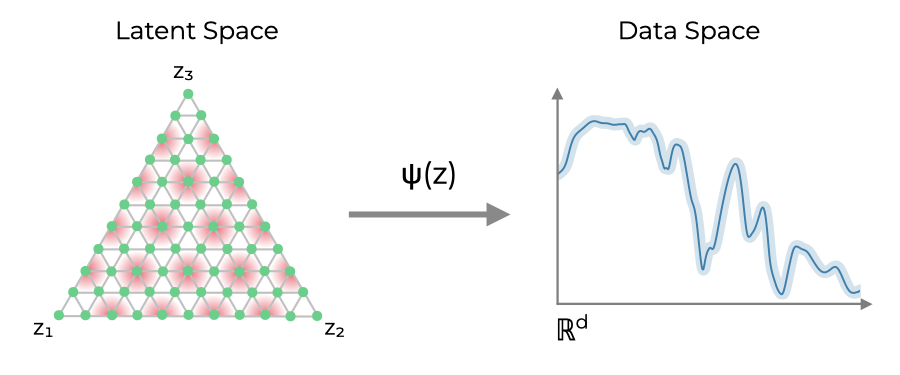
\includegraphics[width=\columnwidth]{figures/methods/gsm-diagram.png}
\caption{ \label{fig:gsm-diagram}}
\end{figure}  


\subsection{Implementation Details}

The mixing coefficients are initially chosen so that $\pi_k = \frac{1}{K}$.

- Linear Method

- Nonlinear Method

- Mixed Method


\section{Experiments}
\subsection{Linear Mixing: Comparison to NMF}
- describe USGS data
- describe NMF method (for comparisson)
- describe evaluation criteria

\subsection{Nonlinear Mixing: Water Contaminant Identification}
- describe robot team data collection and processing
- describe 

\section{Results}
\subsection{Linear Mixing}
\subsection{Nonlinear Mixing: Rhodamine Dye Plume}
\subsection{Nonlinear Mixing: Semi-supervised Analysis}


\section{Discussion}

- Comparison to NMF on linear mixing problem
    - note that there are many versions of NMF with different constraints/regularization. The purpose here was to show that GSM is at least \textit{comparable} to NMF for linear unmixing problems
    - Further note that both NMF and GSM do not rely on assumption of pure pixels (unlike VCA and other methods) 
    - GSM also allows estimation of endmember variability via the precision parameter $\beta$ i.e. nodes in data space follow Gaussian distribution with $\sigma = \sqrt{\beta^{-1}}$

- Nonlinear GSM for robot team 
    - discuss identification of rhodamine plume and easy abundance mapping via the embedding coordinate
    - discuss intrinsic dimensionality identification via abundance sparsity and BIC
    - Discuss identification of non-linearity \textit{strength} via regularization parameter and BIC.
    - reconstruction rmse can also be used to evaluate the relative performance for fixed model size (i.e. k and m) with varying regularization strength

- Limitations of the GSM
    - slow training due to computation of dinstance matrix between full dataset and embedding space
    - An incremental version of the EM procedure as described in \cite{gtm-developments} can speed this up by considering batches $X_b$ of $X$ and performing only a partial E-step by updating responsibilities corresponding to the data batch
    - However, M step still involves the "full" responsibility matrix. 
    - This can be addressed by taking an ensembling approach as described in \cite{parallel-gtm} where multiple GTM are trained on subsets of $X$ and the results are averaged. 
    - More generally, we may consider a mixture-of-GTMs as briefly desribed in \cite{gtm-orig} whereby the overall density is given as 
    \begin{equation}
        p(\mathbf{x}) = \sum_r P(r)p(\mathbf{x}\vert r)
    \end{equation}
    where there are $r$ individual GTM models with mixing coefficients $P(r)$ such that $\sum_r P(r) =1$

- Other potential extensions to GSM model
     - Adapt latent space  to allow for points whose barycentric coordinates sum to less than 1 in order to account for lighting effects (shouldn't matter for reflectance but would matter for radiance depending on incident light). This is the $\gamma$ factor that shows up in some of the mixing papers.

- Discuss other applications of the GSM
    - Optimal route planning for in-situ data collection based on prize-collecting travelling salesman problem, i.e. construct a route which maximizies area traversed in GSM latent space (e.g. the n-simplex). 
    - Applications to source apportionment, e.g. linear GSM can be used for standard source apportionment problems (no reactions) and nonlinear GSM may be useful for modeling scenarios with aditional complications due to reactions and transfport from source to receptor.

\section{Conclusions}


\section{Patents}

\textcolor{red}{UPDATE ME!}

%%%%%%%%%%%%%%%%%%%%%%%%%%%%%%%%%%%%%%%%%%
\vspace{6pt} 


%%%%%%%%%%%%%%%%%%%%%%%%%%%%%%%%%%%%%%%%%%
\authorcontributions{Methodology, J.W.; conceptualization, J.W.; software, J.W.; validation, J.W.; formal analysis, J.W.; investigation J.W.; resources, D.J.L.; writing---original draft preparation, J.W.; writing---review and editing, J.W. and D.J.L.; visualization, J.W.; supervision, D.J.L.; project administration, D.J.L.; funding acquisition, D.J.L. All authors have read and agreed to the published version of the manuscript.
}


\funding{\textcolor{red}{Please add: ``This research received no external funding'' or ``This research was funded by NAME OF FUNDER grant number XXX.'' and  and ``The APC was funded by XXX''. Check carefully that the details given are accurate and use the standard spelling of funding agency names at \url{https://search.crossref.org/funding}, any errors may affect your future funding.}}


\institutionalreview{Not applicable.}

\informedconsent{Not applicable.}


\dataavailability{\textcolor{red}{We encourage all authors of articles published in MDPI journals to share their research data. In this section, please provide details regarding where data supporting reported results can be found, including links to publicly archived datasets analyzed or generated during the study. Where no new data were created, or where data is unavailable due to privacy or ethical restrictions, a statement is still required. Suggested Data Availability Statements are available in section ``MDPI Research Data Policies'' at \url{https://www.mdpi.com/ethics}.}}


\acknowledgments{\textcolor{red}{In this section you can acknowledge any support given which is not covered by the author contribution or funding sections. This may include administrative and technical support, or donations in kind (e.g., materials used for experiments).}}

\conflictsofinterest{The authors declare no conflicts of interest.}
 

%%%%%%%%%%%%%%%%%%%%%%%%%%%%%%%%%%%%%%%%%%
%% Optional

%% Only for journal Encyclopedia
%\entrylink{The Link to this entry published on the encyclopedia platform.}

\abbreviations{Abbreviations}{
The following abbreviations are used in this manuscript:\\

\noindent 
\begin{tabular}{@{}ll}
MDPI & Multidisciplinary Digital Publishing Institute\\
DOAJ & Directory of open access journals\\
TLA & Three letter acronym\\
LD & Linear dichroism
\end{tabular}
}

%%%%%%%%%%%%%%%%%%%%%%%%%%%%%%%%%%%%%%%%%%
%% Optional
\appendixtitles{no} % Leave argument "no" if all appendix headings stay EMPTY (then no dot is printed after "Appendix A"). If the appendix sections contain a heading then change the argument to "yes".


%%%%%%%%%%%%%%%%%%%%%%%%%%%%%%%%%%%%%%%%%%
\begin{adjustwidth}{-\extralength}{0cm}
%\printendnotes[custom] % Un-comment to print a list of endnotes

\reftitle{References}

\bibliography{paper/references}
\PublishersNote{}

\end{adjustwidth}
\end{document}

